% =========================================================
% BORRADOR (NO INCLUIDO EN main.tex TODAVÍA)
% Estructura de Resultados, Discusión y Conclusiones, sin cifras.
% Creado el 9 de noviembre de 2026, antes de terminar la ejecución principal.
%
% Cómo usarlo cuando existan resultados:
%   1. python Experimentos/generar_resultados_latex.py <carpeta con results.csv>
%      (escribe tablas y figura en Manuscrito/resultados_generados/).
%   2. Añadir \usepackage{graphicx} al preámbulo de main.tex.
%   3. Copiar este contenido a main.tex, sustituyendo cada bloque «COMPLETAR»
%      por texto redactado con los números reales. No dejar afirmaciones
%      que los datos no respalden.
% Reglas del proyecto: voz impersonal, español académico sencillo y prudente;
% hipótesis y clasificación no son causalidad; tres cadenas no permiten
% inferencia general; no tratar los textos como réplicas independientes.
% =========================================================

\section{Resultados}

\subsection{Ejecución realizada y verificación de los datos}
% COMPLETAR con hechos verificables de verificacion_y_valores.json:
% - etapas completadas (48 previstas) y entorno efectivo (GPU, versiones);
% - fecha y duración aproximada de la ejecución;
% - longitud léxica W fijada con validación;
% - textos más cortos que W y truncamientos del codificador (si los hubo);
% - cualquier desviación respecto del protocolo y su causa.

\subsection{Trayectorias de las métricas}
% COMPLETAR: describir, sin interpretar causas, cómo cambian las cinco métricas
% por ciclo y proporción sintética. Referenciar la figura y las tablas:
%   % Generado por Experimentos/generar_resultados_latex.py desde complementario.
% No editar a mano: volver a ejecutar el script.

\begin{table}[ht]
\centering
\footnotesize
\begin{tabular}{c c c c}
\hline
Ciclo & $\alpha=0$ & $\alpha=0.5$ & $\alpha=1$ \\
\hline
0 ($M_0$) & \multicolumn{3}{c}{$30.46$ [$30.40$; $30.51$]} \\
1 & $30.49$ [$30.46$; $30.52$] & $31.61$ [$31.45$; $31.76$] & $32.92$ [$32.81$; $33.00$] \\
2 & $30.46$ [$30.32$; $30.57$] & $31.87$ [$31.57$; $32.03$] & $34.46$ [$34.33$; $34.73$] \\
3 & $30.47$ [$30.43$; $30.51$] & $31.86$ [$31.75$; $32.06$] & $36.11$ [$35.74$; $36.32$] \\
4 & $30.40$ [$30.38$; $30.42$] & $31.90$ [$31.85$; $31.96$] & $38.03$ [$37.73$; $38.53$] \\
5 & $30.47$ [$30.40$; $30.51$] & $31.90$ [$31.69$; $32.18$] & $39.30$ [$39.01$; $39.76$] \\
\hline
\end{tabular}
\caption{Perplejidad sobre referencias originales: media y rango [mínimo; máximo] de las tres cadenas por ciclo y proporción sintética $\alpha$. $M_0$ es compartido por las tres proporciones dentro de cada repetición. Salvo la perplejidad, calculada con los 128 contextos de prueba, las métricas corresponden al análisis complementario \textit{post hoc} con los 90 contextos en los que todas las etapas alcanzan $W=30$ palabras.}
\label{tab:medias_human_perplexity}
\end{table}

%   % Generado por Experimentos/generar_resultados_latex.py desde complementario.
% No editar a mano: volver a ejecutar el script.

\begin{table}[ht]
\centering
\footnotesize
\begin{tabular}{c c c c}
\hline
Ciclo & $\alpha=0$ & $\alpha=0.5$ & $\alpha=1$ \\
\hline
0 ($M_0$) & \multicolumn{3}{c}{$0.9133$ [$0.9111$; $0.9169$]} \\
1 & $0.9064$ [$0.9038$; $0.9077$] & $0.8981$ [$0.8958$; $0.8996$] & $0.8944$ [$0.8854$; $0.9057$] \\
2 & $0.9022$ [$0.8989$; $0.9050$] & $0.8962$ [$0.8793$; $0.9084$] & $0.8779$ [$0.8716$; $0.8874$] \\
3 & $0.9170$ [$0.9115$; $0.9226$] & $0.9000$ [$0.8900$; $0.9103$] & $0.8479$ [$0.8460$; $0.8498$] \\
4 & $0.9197$ [$0.9115$; $0.9310$] & $0.9017$ [$0.8908$; $0.9115$] & $0.8341$ [$0.8284$; $0.8372$] \\
5 & $0.9050$ [$0.8985$; $0.9142$] & $0.8959$ [$0.8900$; $0.9023$] & $0.8250$ [$0.8153$; $0.8349$] \\
\hline
\end{tabular}
\caption{Distinct-2: media y rango [mínimo; máximo] de las tres cadenas por ciclo y proporción sintética $\alpha$. $M_0$ es compartido por las tres proporciones dentro de cada repetición. Salvo la perplejidad, calculada con los 128 contextos de prueba, las métricas corresponden al análisis complementario \textit{post hoc} con los 90 contextos en los que todas las etapas alcanzan $W=30$ palabras.}
\label{tab:medias_distinct_2}
\end{table}

%   % Generado por Experimentos/generar_resultados_latex.py desde complementario.
% No editar a mano: volver a ejecutar el script.

\begin{table}[ht]
\centering
\footnotesize
\begin{tabular}{c c c c}
\hline
Ciclo & $\alpha=0$ & $\alpha=0.5$ & $\alpha=1$ \\
\hline
0 ($M_0$) & \multicolumn{3}{c}{$0.9896$ [$0.9841$; $0.9933$]} \\
1 & $0.9839$ [$0.9813$; $0.9877$] & $0.9839$ [$0.9817$; $0.9849$] & $0.9831$ [$0.9802$; $0.9853$] \\
2 & $0.9837$ [$0.9786$; $0.9865$] & $0.9865$ [$0.9802$; $0.9909$] & $0.9721$ [$0.9663$; $0.9782$] \\
3 & $0.9893$ [$0.9853$; $0.9925$] & $0.9856$ [$0.9806$; $0.9909$] & $0.9532$ [$0.9508$; $0.9567$] \\
4 & $0.9877$ [$0.9833$; $0.9913$] & $0.9849$ [$0.9810$; $0.9881$] & $0.9529$ [$0.9484$; $0.9575$] \\
5 & $0.9854$ [$0.9837$; $0.9877$] & $0.9839$ [$0.9778$; $0.9877$] & $0.9401$ [$0.9357$; $0.9476$] \\
\hline
\end{tabular}
\caption{Distinct-3: media y rango [mínimo; máximo] de las tres cadenas por ciclo y proporción sintética $\alpha$. $M_0$ es compartido por las tres proporciones dentro de cada repetición. Salvo la perplejidad, calculada con los 128 contextos de prueba, las métricas corresponden al análisis complementario \textit{post hoc} con los 90 contextos en los que todas las etapas alcanzan $W=30$ palabras.}
\label{tab:medias_distinct_3}
\end{table}

%   % Generado por Experimentos/generar_resultados_latex.py desde complementario.
% No editar a mano: volver a ejecutar el script.

\begin{table}[ht]
\centering
\footnotesize
\begin{tabular}{c c c c}
\hline
Ciclo & $\alpha=0$ & $\alpha=0.5$ & $\alpha=1$ \\
\hline
0 ($M_0$) & \multicolumn{3}{c}{$0.0030$ [$0.0012$; $0.0062$]} \\
1 & $0.0053$ [$0.0029$; $0.0070$] & $0.0044$ [$0.0025$; $0.0066$] & $0.0051$ [$0.0025$; $0.0066$] \\
2 & $0.0059$ [$0.0021$; $0.0123$] & $0.0032$ [$0.0004$; $0.0066$] & $0.0140$ [$0.0074$; $0.0206$] \\
3 & $0.0030$ [$0.0012$; $0.0045$] & $0.0043$ [$0.0012$; $0.0066$] & $0.0261$ [$0.0206$; $0.0288$] \\
4 & $0.0047$ [$0.0021$; $0.0070$] & $0.0052$ [$0.0016$; $0.0074$] & $0.0225$ [$0.0198$; $0.0272$] \\
5 & $0.0043$ [$0.0033$; $0.0049$] & $0.0048$ [$0.0025$; $0.0091$] & $0.0350$ [$0.0276$; $0.0387$] \\
\hline
\end{tabular}
\caption{Repetición media de 4-gramas: media y rango [mínimo; máximo] de las tres cadenas por ciclo y proporción sintética $\alpha$. $M_0$ es compartido por las tres proporciones dentro de cada repetición. Salvo la perplejidad, calculada con los 128 contextos de prueba, las métricas corresponden al análisis complementario \textit{post hoc} con los 90 contextos en los que todas las etapas alcanzan $W=30$ palabras.}
\label{tab:medias_repeat_4_mean}
\end{table}

%   % Generado por Experimentos/generar_resultados_latex.py desde complementario.
% No editar a mano: volver a ejecutar el script.

\begin{table}[ht]
\centering
\footnotesize
\begin{tabular}{c c c c}
\hline
Ciclo & $\alpha=0$ & $\alpha=0.5$ & $\alpha=1$ \\
\hline
0 ($M_0$) & \multicolumn{3}{c}{$0.8827$ [$0.8752$; $0.8901$]} \\
1 & $0.8863$ [$0.8799$; $0.8949$] & $0.8859$ [$0.8739$; $0.8942$] & $0.8864$ [$0.8777$; $0.8939$] \\
2 & $0.8898$ [$0.8861$; $0.8942$] & $0.8954$ [$0.8909$; $0.8982$] & $0.8918$ [$0.8825$; $0.8980$] \\
3 & $0.8886$ [$0.8816$; $0.9009$] & $0.8873$ [$0.8815$; $0.8904$] & $0.8994$ [$0.8934$; $0.9063$] \\
4 & $0.8945$ [$0.8883$; $0.9059$] & $0.8948$ [$0.8941$; $0.8957$] & $0.9017$ [$0.8923$; $0.9066$] \\
5 & $0.8903$ [$0.8862$; $0.8974$] & $0.8984$ [$0.8925$; $0.9018$] & $0.9029$ [$0.9017$; $0.9039$] \\
\hline
\end{tabular}
\caption{Dispersión semántica: media y rango [mínimo; máximo] de las tres cadenas por ciclo y proporción sintética $\alpha$. $M_0$ es compartido por las tres proporciones dentro de cada repetición. Salvo la perplejidad, calculada con los 128 contextos de prueba, las métricas corresponden al análisis complementario \textit{post hoc} con los 90 contextos en los que todas las etapas alcanzan $W=30$ palabras.}
\label{tab:medias_semantic_dispersion}
\end{table}

% Figura:
%   \begin{figure}[ht]\centering
%   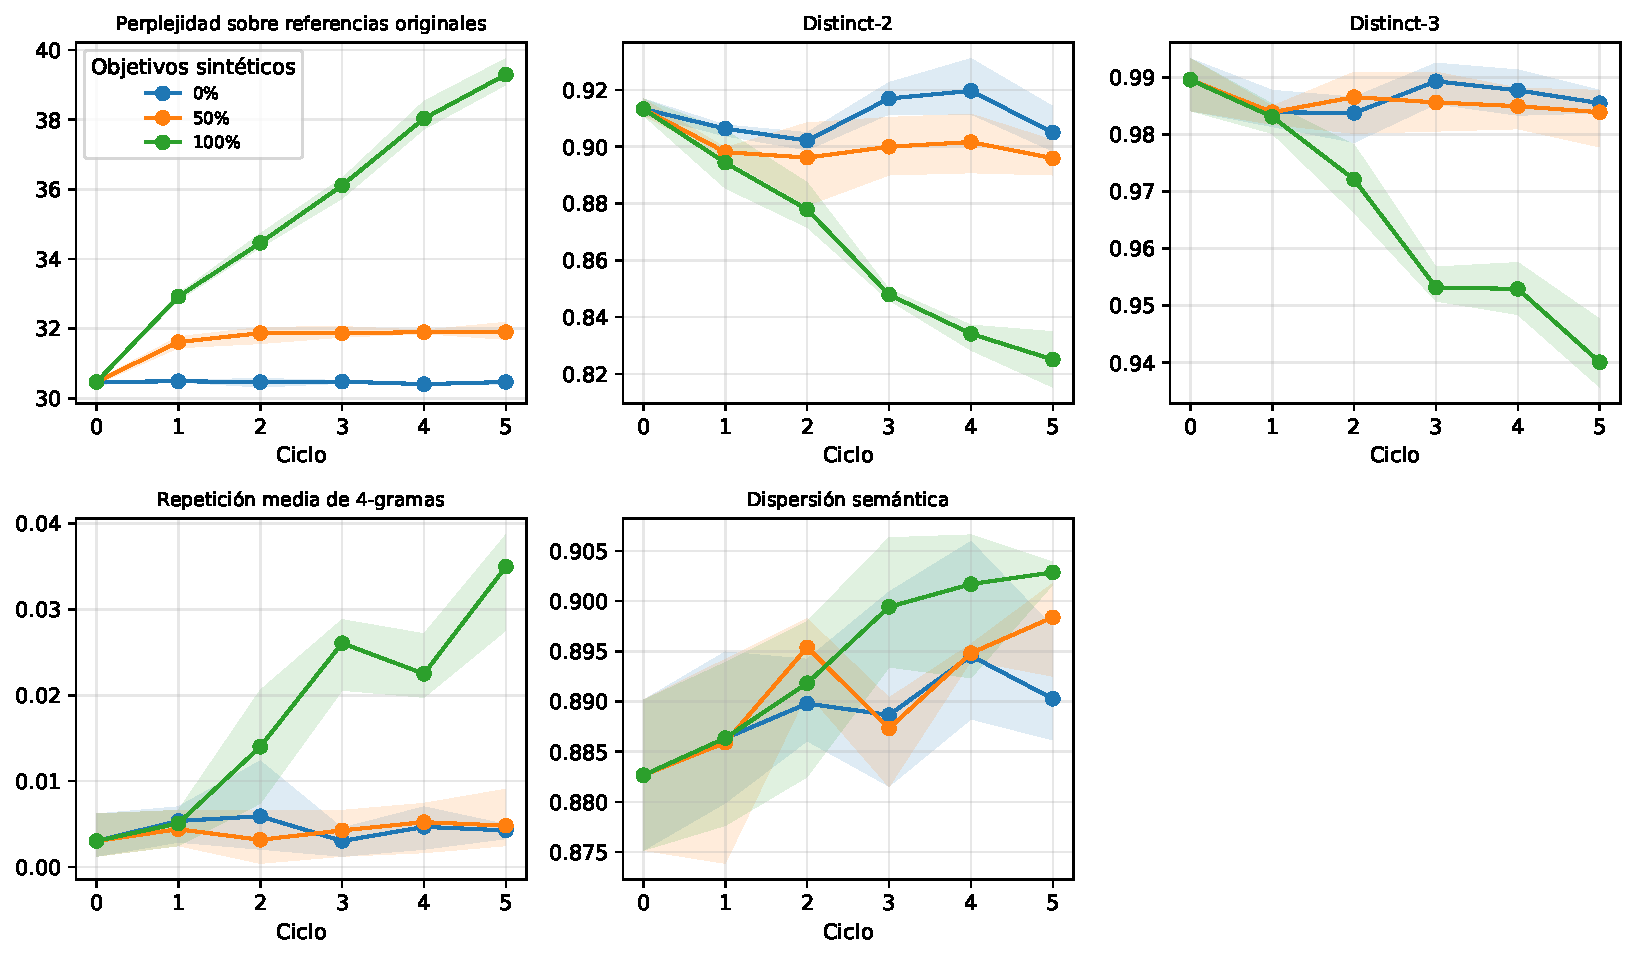
\includegraphics[width=\textwidth]{resultados_generados/figura_trayectorias.pdf}
%   \caption{Media y rango de tres cadenas por ciclo y proporción sintética.}
%   \label{fig:trayectorias}\end{figure}

\subsection{Comparaciones frente al punto inicial y al control}
% COMPLETAR: usar resultados_generados/tabla_contrastes.tex (ciclo final) y, si
% es útil, los contrastes por ciclo de contrasts.csv. Indicar en cuántas de las
% tres cadenas coincide el signo del cambio. Sin p-valores ni «significativo».

\subsection{Muestras de texto generado}
% COMPLETAR: citar con prudencia algunos ejemplos tomados por orden guardado
% (no seleccionados por ser llamativos), indicando etapa y semilla; señalar
% coherencia, repeticiones o caracteres anómalos observados.

\section{Discusión}

\subsection{Lectura de los resultados frente a las preguntas e hipótesis}
% COMPLETAR: relacionar lo observado con cada pregunta de investigación.
% Si no hay deterioro apreciable, decirlo; si lo hay, decir en qué métricas,
% con qué magnitud y con qué consistencia entre cadenas.

\subsection{Comparación con la literatura revisada}
% COMPLETAR: contrastar con los antecedentes del estado del arte (Shumailov,
% Kazdan, Gerstgrasser, etc.) señalando diferencias de protocolo (cada ciclo
% parte del modelo preentrenado, una época, presupuesto fijo, mezcla solo en
% objetivos, contextos humanos fijos). No reclamar novedad.

\subsection{Limitaciones}
% COMPLETAR, conservando lo que ya se declaró en la metodología:
% - tres cadenas y un solo modelo pequeño, idioma y fuente (Wikipedia);
% - ajuste breve desde el modelo preentrenado, no acumulativo;
% - referencia de Wikipedia sin certificación de autoría humana individual
%   y posible solapamiento con el preentrenamiento del generador;
% - métricas de diversidad no miden calidad ni pérdida de patrones raros;
% - sin evaluación humana sistemática;
% - comparaciones exploratorias.

\section{Conclusiones}
% COMPLETAR: respuestas breves a las preguntas, ligadas a lo medido, sin
% generalizar más allá del diseño. Opcional: dos o tres líneas de trabajo
% futuro (acumulación de datos, más repeticiones, evaluación de patrones
% raros, evaluación humana), sin presentarlas como compromisos.
